\documentclass[12pt]{article}

\usepackage{amsmath,amssymb,amsthm}
\usepackage{graphicx}
\usepackage[utf8]{inputenc}
\usepackage{hyperref}
\usepackage{cleveref}
\usepackage{graphicx}
\usepackage{float}



\title{Nash Cipher: A Formal Security Analysis}
\author{Your Name}
\date{\today}

\begin{document}

\maketitle

\begin{abstract}
This document presents a formal analysis of John Nash's encryption system, including mathematical foundations, security properties, and practical implementation considerations.
\end{abstract}

\tableofcontents

\section{Introduction}
\section*{Historical Context}

In 1955, John Nash wrote a series of letters to the NSA describing a novel encryption machine. 
This machine, which we now call the Nash Cipher, demonstrated remarkable foresight in several areas 
of cryptographic design, including:

\begin{itemize}
    \item The concept of computational security
    \item The relationship between key length and security
    \item The importance of complexity in cryptographic transformations
    \item Auto-synchronization in stream ciphers
\end{itemize}

\section*{Document Structure}

This document provides a comprehensive analysis of the Nash Cipher, including:

\begin{itemize}
    \item A formal mathematical description of the cipher
    \item Security analysis and computational hardness arguments
    \item Implementation considerations and practical aspects
    \item Test vectors and verification methodology
\end{itemize}

Our analysis uses modern cryptographic tools and formal methods to evaluate Nash's original design,
including Cryptol specifications and formal verification of security properties.

\section{Mathematical Foundations}
\section*{Mathematical Structure}

The Nash cipher is fundamentally based on a permuter system with the following key mathematical properties:

\begin{enumerate}
    \item Two sets of permutations (red and blue) operating on a binary message stream
    \item Each permutation includes both positional changes and bit transformations
    \item Auto-synchronizing behavior through feedback mechanisms
    \item Cryptographic strength derived from permutation complexity
\end{enumerate}

\section*{Permutation Groups}

The permuter operation can be formalized as follows:

For a permuter with $n$ storage points, each permutation $\pi$ is composed of:
\begin{itemize}
    \item A state transition function $\sigma : \{1,\ldots,n\} \rightarrow \{1,\ldots,n\}$
    \item A bit transformation function $\tau : \{0,1\} \rightarrow \{0,1\}$
\end{itemize}

The total key space is thus:
\[ |K| = \left[n! \cdot 2^{(n+1)}\right]^2 \]

where the square term comes from having both red and blue permutations.

\section*{Security Foundation}

Nash's key insight was that for sufficiently complex permutations, the computational work required to determine the key should grow exponentially with the key length. We can formalize this as:

\[ W(k) = O(2^{c|k|}) \]

where:
\begin{itemize}
    \item $W(k)$ is the work required to determine key $k$
    \item $|k|$ is the bit length of the key
    \item $c$ is some positive constant
\end{itemize}

This exponential growth in computational complexity forms the basis for the cipher's security.

\section{Security Analysis}
\input{chapters/security_analysis}

\section{Implementation}

\section{System Architecture}

\subsection{Permuter Design}
The Nash cipher's core component is a permuter that implements two different state transition paths, labeled as ``red'' and ``blue''. Each path includes both state transitions and bit transformations.

\begin{figure}[H]
    \centering
    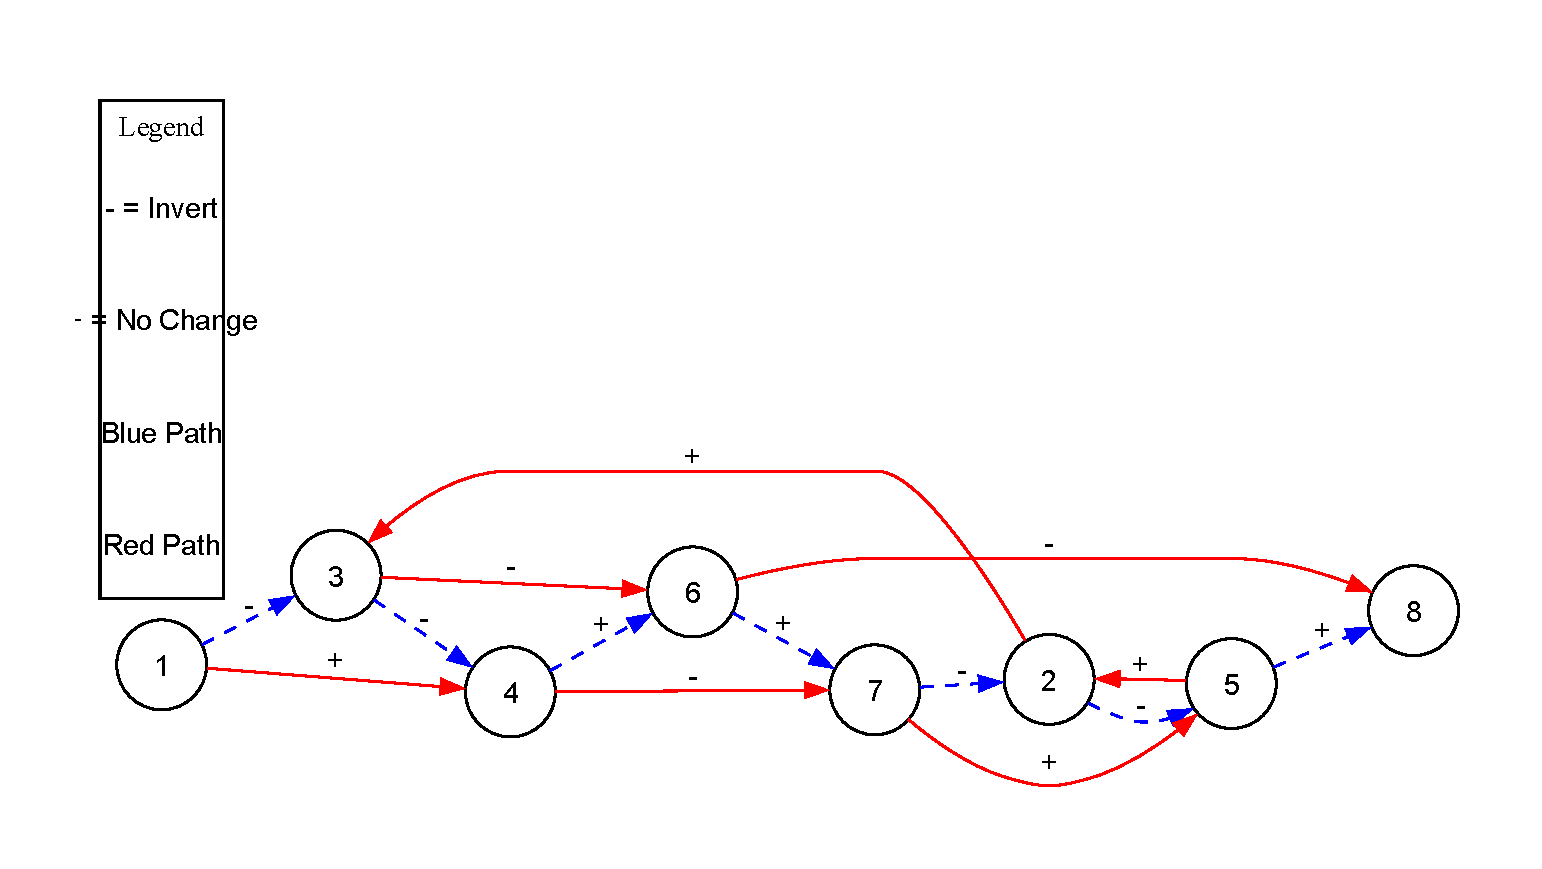
\includegraphics[width=0.8\textwidth]{figures/permuter.pdf}
    \caption{Nash Permuter State Machine. Red (solid) and blue (dashed) paths show different state transitions. The + and - labels indicate whether the bit is preserved or inverted during transition.}
    \label{fig:permuter}
\end{figure}

\subsection{Transmitting Arrangement}
The transmitting arrangement combines the permuter with a feedback mechanism through an adder (binary addition modulo 2) and a decider that selects between red and blue permutation paths.

\begin{figure}[H]
    \centering
    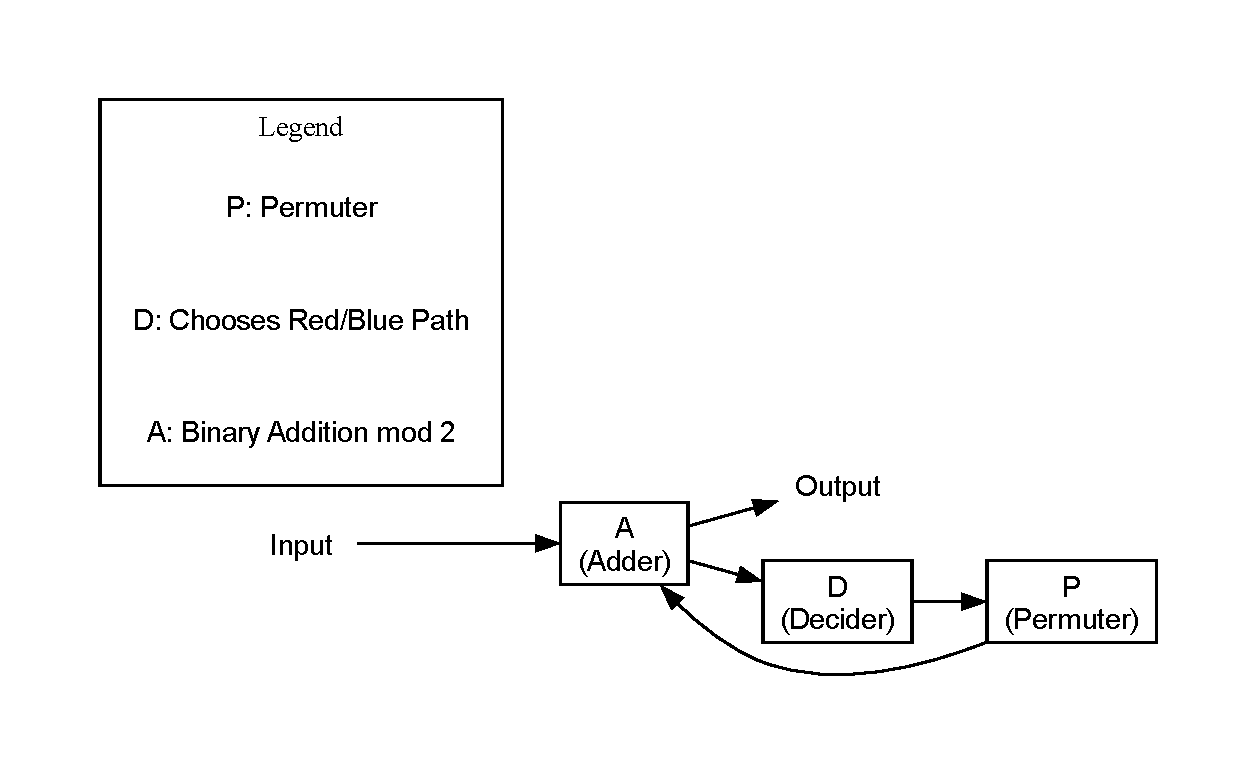
\includegraphics[width=0.8\textwidth]{figures/transmitter.pdf}
    \caption{Nash Cipher Transmitting Arrangement. The adder A performs binary addition modulo 2, decider D selects between red and blue permutation paths based on the adder output, and permuter P performs the state transitions and bit transformations.}
    \label{fig:transmitter}
\end{figure}

\subsection{Receiving Arrangement}
The receiving arrangement mirrors the transmitting arrangement but includes a retarder (one-unit delay) to synchronize the input with the permuter output.

\begin{figure}[H]
    \centering
    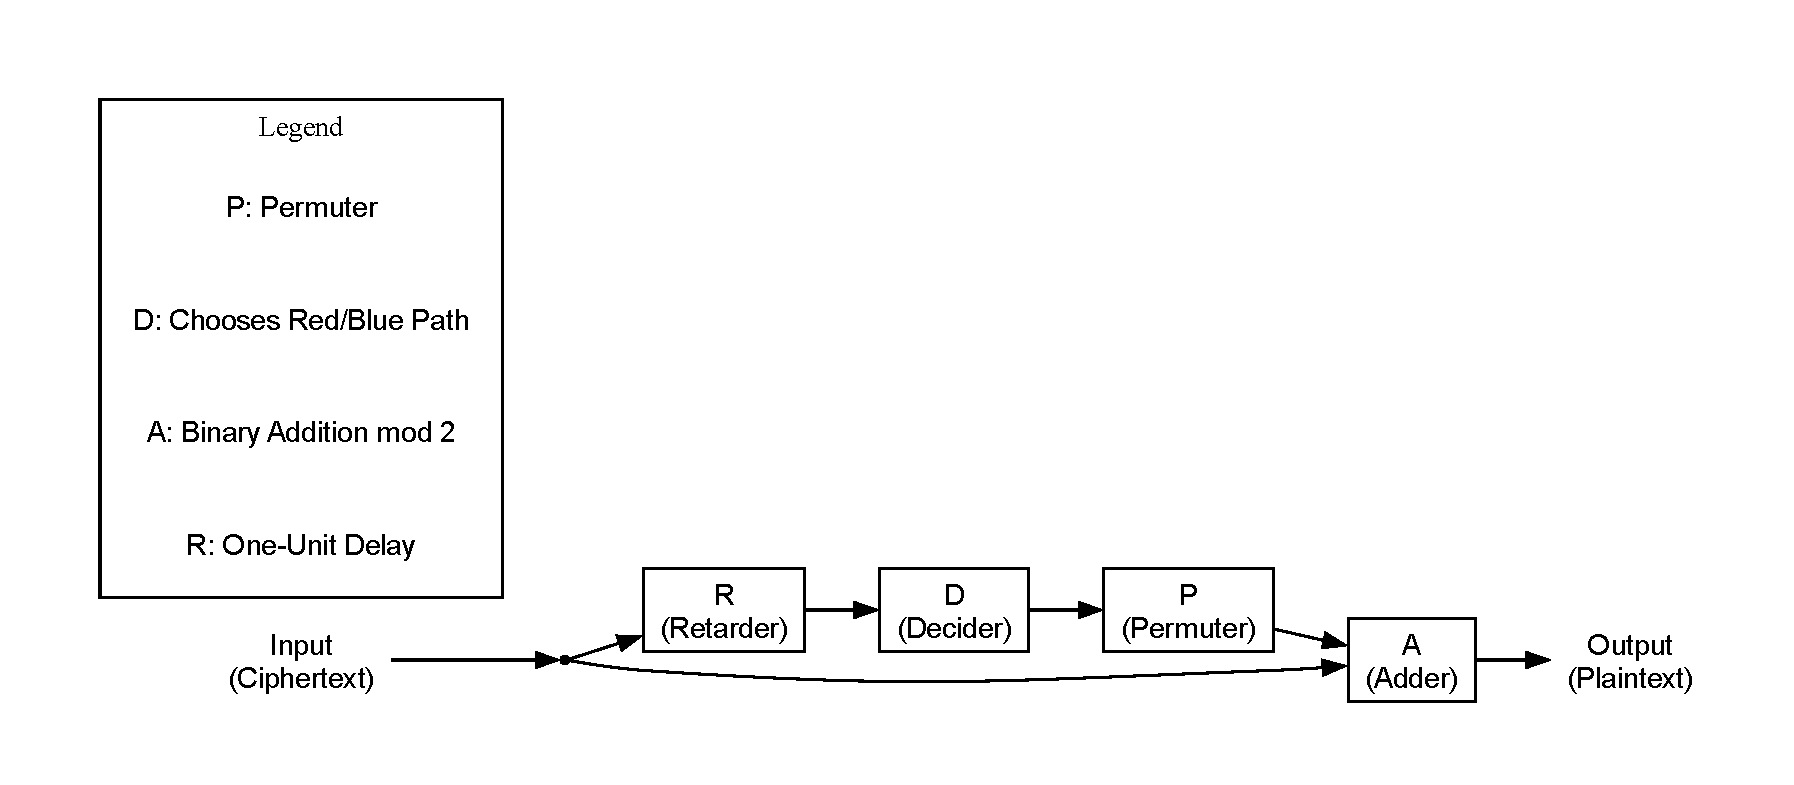
\includegraphics[width=0.8\textwidth]{figures/receiver.pdf}
    \caption{Nash Cipher Receiving Arrangement. The retarder R provides a one-unit delay to synchronize the input with the permuter output. The remaining components function identically to the transmitting arrangement.}
    \label{fig:receiver}
\end{figure}

\section{Key Structure}

The implementation accepts 128-bit keys formatted as hexadecimal values. The key space is structured as follows:

\begin{itemize}
    \item First 64 bits: Red permutation table
    \begin{itemize}
        \item Bits 0-31: Next state mappings
        \item Bits 32-63: Transform functions
    \end{itemize}
    \item Last 64 bits: Blue permutation table
    \begin{itemize}
        \item Bits 64-95: Next state mappings
        \item Bits 96-127: Transform functions
    \end{itemize}
\end{itemize}

\subsection{Key Validation}

Each key must satisfy the following requirements:
\begin{enumerate}
    \item All next state values must be valid (0-7)
    \item Transform functions must be binary (0 or 1)
    \item State transitions must form complete cycles
\end{enumerate}

\subsection{Example Key Format}
Keys are represented in hexadecimal format:
\begin{verbatim}
[<:AA9987E016931D993B2359B1103A88C6:>]
\end{verbatim}

This notation ensures consistent key handling across different implementations while maintaining compatibility with standard cryptographic interfaces.

\section{Implementation Considerations}

\subsection{State Machine Implementation}
The cipher's state machine requires...

[Note: Additional implementation details to be added]

\section{Test Vectors}
\input{chapters/test_vectors}

\bibliographystyle{plain}
\bibliography{bibliography}

\end{document}